\chapter{Introduction}

The Research Institute Řež conducts numerous projects within the nuclear industry, many of which involve electron microscopy and the analysis of materials exposed to high temperatures and aggressive environments, such as those found in nuclear reactors. A significant portion of these projects requires extensive manual image analysis, making automation a key challenge. Currently, image analysis is performed using various processing tools, including Fiji~\cite{Schindelin2012} by ImageJ. This thesis aims to automate one of these manual processes.

The images analyzed in this thesis are part of a project that includes two main image categories: material samples with protective coating layers and samples with extensive oxidation and no coating. This work focuses exclusively on the coated samples, which typically exhibit more uniform and structured features compared to the irregular and heterogeneous appearance of the oxidized samples. Examples of both image types are shown in Figure~\ref{fig:coating-oxidation}. The coated images originate from a study investigating the thickness and integrity of cladding layers applied to various materials, both before and after exposure to high temperatures and aggressive environments, with the aim of evaluating their protective performance. This thesis focuses on the automated measurement of the coating layers. Although the current work is limited to coated samples, the methods developed here may later be adapted for use with the more complex oxidized samples.


To address the segmentation task, three computer vision approaches are explored, ranging from traditional clustering methods to advanced deep learning models. The first method investigated is K-means clustering, an unsupervised algorithm that does not require labeled data. Although K-means offers a lightweight and accessible approach, its performance is constrained by the complex and non-homogeneous nature of the coating layers. Variability in layer structure, color, and visual features requires image-specific parameter tuning, which limits its general usability. A more detailed evaluation of this method is presented in Section~\ref{sec:kmeans}.



\begin{figure}[H]
    \centering
    \begin{subfigure}{0.4\textwidth}
        \centering
        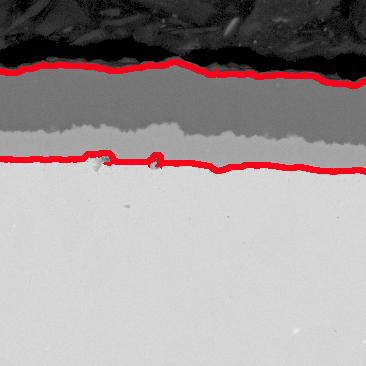
\includegraphics[width=\linewidth]{PICTURES/intro/177_CROP.png}
        \caption{Cropped image showing a protective coating layer highlighted in red.}         
        \label{fig:coating}
    \end{subfigure}
    \hfill
    \begin{subfigure}{0.4\textwidth}
        \centering
        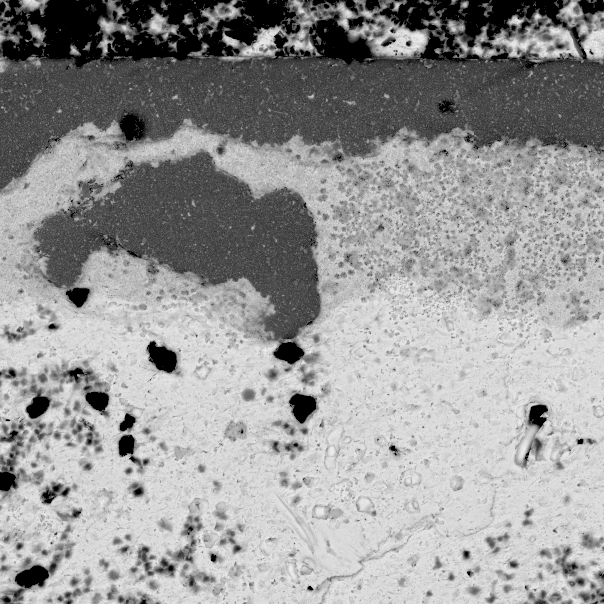
\includegraphics[width=\linewidth]{PICTURES/intro/625_3500h_low_cross_strana1_13_crop.png}
     \caption{Cropped image of a sample exhibiting oxidation without coating.} \label{fig:oxidation}        
     \label{fig:oxidation}
    \end{subfigure}
    \caption{Examples of coating and oxidation layers in material samples.}
    \label{fig:coating-oxidation}
\end{figure}


The second method involves the Segment Anything Model (SAM)\cite{kirillov2023segany}, a state-of-the-art segmentation approach based on transformers. SAM is designed for general-purpose segmentation and demonstrates considerable potential due to its flexibility and robust architecture. However, it requires significantly higher computational resources and, in practice, was found to lack the specificity and precision needed for accurate segmentation of coating and oxidation layers. This limitation is further analyzed in Section~\ref{sec:sam}.

The third approach utilizes Convolutional Neural Networks (CNNs), which demand labeled training data but are capable of achieving high segmentation accuracy once trained. In this work, three types of labels were developed for training and evaluation. Initially, no ground truth annotations were available. To address this, the Fiji image processing software—commonly used by scientists for manual analysis—was modified to support manual annotation while capturing precise measurement data. This enhancement enabled the creation of the first type of labels: polygon-based annotations.

During the manual annotation process, the results from a previous experiment using K-means clustering were collected to generate a second dataset. However, K-means struggled to reliably distinguish between coating and oxidation, especially in more complex cases. To address this, a third label type, called refined K-means, was introduced. These labels were manually adjusted versions of the K-means labels, corrected and improved using image editing tools by researchers. This final set of labels represents the most accurate annotations and serves as the ground truth for evaluating the CNN models. A more detailed discussion on the CNN approach and label development is provided in Section~\ref{sec:cnn}.

Following the creation of the label sets, a CNN model was developed and trained using the refined K-means annotations. The model underwent hyperparameter tuning to optimize its performance. For comparison, additional models were trained on the first and second label types to estimate their expected performance in future applications.

The final model was evaluated not only on a dedicated test dataset but also in a practical setting by researchers. This evaluation considered both segmentation accuracy and the time required for image analysis, as discussed in Sections~\ref{sec:res} and~\ref{sec:resprec}. Given the limited size of the initial dataset, the long-term goal is to establish a feedback loop: by automating the labeling process, more samples can be efficiently annotated. This expanded dataset would, in turn, allow the model to further improve its performance, continuously enhancing both the speed and accuracy of the image analysis workflow.

This thesis is structured as follows: Sections~\ref{sec:kmeans} and~\ref{sec:sam} discuss the two image segmentation methods and why they could not be implemented. Section~\ref{sec:cnn} discusses label creation and model training based on the CNN approach. Section~\ref{sec:integ} describes the integration of the trained model into the existing labeling software. The results, including analysis of segmentation accuracy and time efficiency, are presented in Sections~\ref{sec:res} and~\ref{sec:resprec}. Finally, Section~\ref{chap:con} concludes the thesis with a summary and a discussion of potential future developments.
